\documentclass[twoside]{book}

% Packages required by doxygen
\usepackage{fixltx2e}
\usepackage{calc}
\usepackage{doxygen}
\usepackage[export]{adjustbox} % also loads graphicx
\usepackage{graphicx}
\usepackage[utf8]{inputenc}
\usepackage{makeidx}
\usepackage{multicol}
\usepackage{multirow}
\PassOptionsToPackage{warn}{textcomp}
\usepackage{textcomp}
\usepackage[nointegrals]{wasysym}
\usepackage[table]{xcolor}

% Font selection
\usepackage[T1]{fontenc}
\usepackage[scaled=.90]{helvet}
\usepackage{courier}
\usepackage{amssymb}
\usepackage{sectsty}
\renewcommand{\familydefault}{\sfdefault}
\allsectionsfont{%
  \fontseries{bc}\selectfont%
  \color{darkgray}%
}
\renewcommand{\DoxyLabelFont}{%
  \fontseries{bc}\selectfont%
  \color{darkgray}%
}
\newcommand{\+}{\discretionary{\mbox{\scriptsize$\hookleftarrow$}}{}{}}

% Page & text layout
\usepackage{geometry}
\geometry{%
  a4paper,%
  top=2.5cm,%
  bottom=2.5cm,%
  left=2.5cm,%
  right=2.5cm%
}
\tolerance=750
\hfuzz=15pt
\hbadness=750
\setlength{\emergencystretch}{15pt}
\setlength{\parindent}{0cm}
\setlength{\parskip}{3ex plus 2ex minus 2ex}
\makeatletter
\renewcommand{\paragraph}{%
  \@startsection{paragraph}{4}{0ex}{-1.0ex}{1.0ex}{%
    \normalfont\normalsize\bfseries\SS@parafont%
  }%
}
\renewcommand{\subparagraph}{%
  \@startsection{subparagraph}{5}{0ex}{-1.0ex}{1.0ex}{%
    \normalfont\normalsize\bfseries\SS@subparafont%
  }%
}
\makeatother

% Headers & footers
\usepackage{fancyhdr}
\pagestyle{fancyplain}
\fancyhead[LE]{\fancyplain{}{\bfseries\thepage}}
\fancyhead[CE]{\fancyplain{}{}}
\fancyhead[RE]{\fancyplain{}{\bfseries\leftmark}}
\fancyhead[LO]{\fancyplain{}{\bfseries\rightmark}}
\fancyhead[CO]{\fancyplain{}{}}
\fancyhead[RO]{\fancyplain{}{\bfseries\thepage}}
\fancyfoot[LE]{\fancyplain{}{}}
\fancyfoot[CE]{\fancyplain{}{}}
\fancyfoot[RE]{\fancyplain{}{\bfseries\scriptsize Generated by Doxygen }}
\fancyfoot[LO]{\fancyplain{}{\bfseries\scriptsize Generated by Doxygen }}
\fancyfoot[CO]{\fancyplain{}{}}
\fancyfoot[RO]{\fancyplain{}{}}
\renewcommand{\footrulewidth}{0.4pt}
\renewcommand{\chaptermark}[1]{%
  \markboth{#1}{}%
}
\renewcommand{\sectionmark}[1]{%
  \markright{\thesection\ #1}%
}

% Indices & bibliography
\usepackage{natbib}
\usepackage[titles]{tocloft}
\setcounter{tocdepth}{3}
\setcounter{secnumdepth}{5}
\makeindex

% Hyperlinks (required, but should be loaded last)
\usepackage{ifpdf}
\ifpdf
  \usepackage[pdftex,pagebackref=true]{hyperref}
\else
  \usepackage[ps2pdf,pagebackref=true]{hyperref}
\fi
\hypersetup{%
  colorlinks=true,%
  linkcolor=blue,%
  citecolor=blue,%
  unicode%
}

% Custom commands
\newcommand{\clearemptydoublepage}{%
  \newpage{\pagestyle{empty}\cleardoublepage}%
}

\usepackage{caption}
\captionsetup{labelsep=space,justification=centering,font={bf},singlelinecheck=off,skip=4pt,position=top}

%===== C O N T E N T S =====

\begin{document}

% Titlepage & ToC
\hypersetup{pageanchor=false,
             bookmarksnumbered=true,
             pdfencoding=unicode
            }
\pagenumbering{alph}
\begin{titlepage}
\vspace*{7cm}
\begin{center}%
{\Large C\+E\+C\+S\+\_\+327\+\_\+\+Lab\+\_\+02 }\\
\vspace*{1cm}
{\large Generated by Doxygen 1.8.13}\\
\end{center}
\end{titlepage}
\clearemptydoublepage
\pagenumbering{roman}
\tableofcontents
\clearemptydoublepage
\pagenumbering{arabic}
\hypersetup{pageanchor=true}

%--- Begin generated contents ---
\chapter{Data Structure Index}
\section{Data Structures}
Here are the data structures with brief descriptions\+:\begin{DoxyCompactList}
\item\contentsline{section}{\hyperlink{structmotion__time__t}{motion\+\_\+time\+\_\+t} }{\pageref{structmotion__time__t}}{}
\item\contentsline{section}{\hyperlink{structnearest__neighbor__t}{nearest\+\_\+neighbor\+\_\+t} }{\pageref{structnearest__neighbor__t}}{}
\item\contentsline{section}{\hyperlink{struct_u_s_e_r_d_a_t_a}{U\+S\+E\+R\+D\+A\+TA} }{\pageref{struct_u_s_e_r_d_a_t_a}}{}
\end{DoxyCompactList}

\chapter{File Index}
\section{File List}
Here is a list of all files with brief descriptions\+:\begin{DoxyCompactList}
\item\contentsline{section}{Assignment1/\hyperlink{ftpclient_8cpp}{ftpclient.\+cpp} }{\pageref{ftpclient_8cpp}}{}
\end{DoxyCompactList}

\chapter{Data Structure Documentation}
\hypertarget{structmotion__time__t}{}\section{motion\+\_\+time\+\_\+t Struct Reference}
\label{structmotion__time__t}\index{motion\+\_\+time\+\_\+t@{motion\+\_\+time\+\_\+t}}


{\ttfamily \#include $<$ring.\+h$>$}

\subsection*{Data Fields}
\begin{DoxyCompactItemize}
\item 
uint8\+\_\+t \hyperlink{structmotion__time__t_af5cce4e990612a7df34e50eab7a2e587}{motion}
\item 
uint8\+\_\+t \hyperlink{structmotion__time__t_a3b4bcf3c4c4d82f8d051e3d08a4c40a3}{time}
\end{DoxyCompactItemize}


\subsection{Field Documentation}
\mbox{\Hypertarget{structmotion__time__t_af5cce4e990612a7df34e50eab7a2e587}\label{structmotion__time__t_af5cce4e990612a7df34e50eab7a2e587}} 
\index{motion\+\_\+time\+\_\+t@{motion\+\_\+time\+\_\+t}!motion@{motion}}
\index{motion@{motion}!motion\+\_\+time\+\_\+t@{motion\+\_\+time\+\_\+t}}
\subsubsection{\texorpdfstring{motion}{motion}}
{\footnotesize\ttfamily uint8\+\_\+t motion}

\mbox{\Hypertarget{structmotion__time__t_a3b4bcf3c4c4d82f8d051e3d08a4c40a3}\label{structmotion__time__t_a3b4bcf3c4c4d82f8d051e3d08a4c40a3}} 
\index{motion\+\_\+time\+\_\+t@{motion\+\_\+time\+\_\+t}!time@{time}}
\index{time@{time}!motion\+\_\+time\+\_\+t@{motion\+\_\+time\+\_\+t}}
\subsubsection{\texorpdfstring{time}{time}}
{\footnotesize\ttfamily uint8\+\_\+t time}



The documentation for this struct was generated from the following file\+:\begin{DoxyCompactItemize}
\item 
\hyperlink{ring_8h}{ring.\+h}\end{DoxyCompactItemize}

\hypertarget{structnearest__neighbor__t}{}\section{nearest\+\_\+neighbor\+\_\+t Struct Reference}
\label{structnearest__neighbor__t}\index{nearest\+\_\+neighbor\+\_\+t@{nearest\+\_\+neighbor\+\_\+t}}


{\ttfamily \#include $<$ring.\+h$>$}

\subsection*{Data Fields}
\begin{DoxyCompactItemize}
\item 
uint8\+\_\+t \hyperlink{structnearest__neighbor__t_a1e6927fa1486224044e568f9c370519b}{id}
\item 
uint8\+\_\+t \hyperlink{structnearest__neighbor__t_ad5aa37b153f535af1fc07cf153ea8b75}{right\+\_\+id}
\item 
uint8\+\_\+t \hyperlink{structnearest__neighbor__t_a4d823b5e183e24190a16da36f00a46fb}{left\+\_\+id}
\item 
\hyperlink{ring_8h_a69b20b1a04c8e4cf3b72851b966259ec}{robot\+\_\+state} \hyperlink{structnearest__neighbor__t_aadbb2fcd5b6edab38e3aa5aca6d92439}{state}
\item 
uint8\+\_\+t \hyperlink{structnearest__neighbor__t_a99ae28d976be4f4b3aada22693153bea}{distance}
\item 
uint8\+\_\+t \hyperlink{structnearest__neighbor__t_abea371f9030e15a5d2a4c181576833d8}{num}
\item 
uint8\+\_\+t \hyperlink{structnearest__neighbor__t_ae24749d410d070a1979d9119a2f67147}{num\+\_\+cooperative}
\end{DoxyCompactItemize}


\subsection{Field Documentation}
\mbox{\Hypertarget{structnearest__neighbor__t_a99ae28d976be4f4b3aada22693153bea}\label{structnearest__neighbor__t_a99ae28d976be4f4b3aada22693153bea}} 
\index{nearest\+\_\+neighbor\+\_\+t@{nearest\+\_\+neighbor\+\_\+t}!distance@{distance}}
\index{distance@{distance}!nearest\+\_\+neighbor\+\_\+t@{nearest\+\_\+neighbor\+\_\+t}}
\subsubsection{\texorpdfstring{distance}{distance}}
{\footnotesize\ttfamily uint8\+\_\+t distance}

\mbox{\Hypertarget{structnearest__neighbor__t_a1e6927fa1486224044e568f9c370519b}\label{structnearest__neighbor__t_a1e6927fa1486224044e568f9c370519b}} 
\index{nearest\+\_\+neighbor\+\_\+t@{nearest\+\_\+neighbor\+\_\+t}!id@{id}}
\index{id@{id}!nearest\+\_\+neighbor\+\_\+t@{nearest\+\_\+neighbor\+\_\+t}}
\subsubsection{\texorpdfstring{id}{id}}
{\footnotesize\ttfamily uint8\+\_\+t id}

\mbox{\Hypertarget{structnearest__neighbor__t_a4d823b5e183e24190a16da36f00a46fb}\label{structnearest__neighbor__t_a4d823b5e183e24190a16da36f00a46fb}} 
\index{nearest\+\_\+neighbor\+\_\+t@{nearest\+\_\+neighbor\+\_\+t}!left\+\_\+id@{left\+\_\+id}}
\index{left\+\_\+id@{left\+\_\+id}!nearest\+\_\+neighbor\+\_\+t@{nearest\+\_\+neighbor\+\_\+t}}
\subsubsection{\texorpdfstring{left\+\_\+id}{left\_id}}
{\footnotesize\ttfamily uint8\+\_\+t left\+\_\+id}

\mbox{\Hypertarget{structnearest__neighbor__t_abea371f9030e15a5d2a4c181576833d8}\label{structnearest__neighbor__t_abea371f9030e15a5d2a4c181576833d8}} 
\index{nearest\+\_\+neighbor\+\_\+t@{nearest\+\_\+neighbor\+\_\+t}!num@{num}}
\index{num@{num}!nearest\+\_\+neighbor\+\_\+t@{nearest\+\_\+neighbor\+\_\+t}}
\subsubsection{\texorpdfstring{num}{num}}
{\footnotesize\ttfamily uint8\+\_\+t num}

\mbox{\Hypertarget{structnearest__neighbor__t_ae24749d410d070a1979d9119a2f67147}\label{structnearest__neighbor__t_ae24749d410d070a1979d9119a2f67147}} 
\index{nearest\+\_\+neighbor\+\_\+t@{nearest\+\_\+neighbor\+\_\+t}!num\+\_\+cooperative@{num\+\_\+cooperative}}
\index{num\+\_\+cooperative@{num\+\_\+cooperative}!nearest\+\_\+neighbor\+\_\+t@{nearest\+\_\+neighbor\+\_\+t}}
\subsubsection{\texorpdfstring{num\+\_\+cooperative}{num\_cooperative}}
{\footnotesize\ttfamily uint8\+\_\+t num\+\_\+cooperative}

\mbox{\Hypertarget{structnearest__neighbor__t_ad5aa37b153f535af1fc07cf153ea8b75}\label{structnearest__neighbor__t_ad5aa37b153f535af1fc07cf153ea8b75}} 
\index{nearest\+\_\+neighbor\+\_\+t@{nearest\+\_\+neighbor\+\_\+t}!right\+\_\+id@{right\+\_\+id}}
\index{right\+\_\+id@{right\+\_\+id}!nearest\+\_\+neighbor\+\_\+t@{nearest\+\_\+neighbor\+\_\+t}}
\subsubsection{\texorpdfstring{right\+\_\+id}{right\_id}}
{\footnotesize\ttfamily uint8\+\_\+t right\+\_\+id}

\mbox{\Hypertarget{structnearest__neighbor__t_aadbb2fcd5b6edab38e3aa5aca6d92439}\label{structnearest__neighbor__t_aadbb2fcd5b6edab38e3aa5aca6d92439}} 
\index{nearest\+\_\+neighbor\+\_\+t@{nearest\+\_\+neighbor\+\_\+t}!state@{state}}
\index{state@{state}!nearest\+\_\+neighbor\+\_\+t@{nearest\+\_\+neighbor\+\_\+t}}
\subsubsection{\texorpdfstring{state}{state}}
{\footnotesize\ttfamily \hyperlink{ring_8h_a69b20b1a04c8e4cf3b72851b966259ec}{robot\+\_\+state} state}



The documentation for this struct was generated from the following file\+:\begin{DoxyCompactItemize}
\item 
\hyperlink{ring_8h}{ring.\+h}\end{DoxyCompactItemize}

\hypertarget{struct_u_s_e_r_d_a_t_a}{}\section{U\+S\+E\+R\+D\+A\+TA Struct Reference}
\label{struct_u_s_e_r_d_a_t_a}\index{U\+S\+E\+R\+D\+A\+TA@{U\+S\+E\+R\+D\+A\+TA}}


{\ttfamily \#include $<$ring.\+h$>$}



Collaboration diagram for U\+S\+E\+R\+D\+A\+TA\+:\nopagebreak
\begin{figure}[H]
\begin{center}
\leavevmode
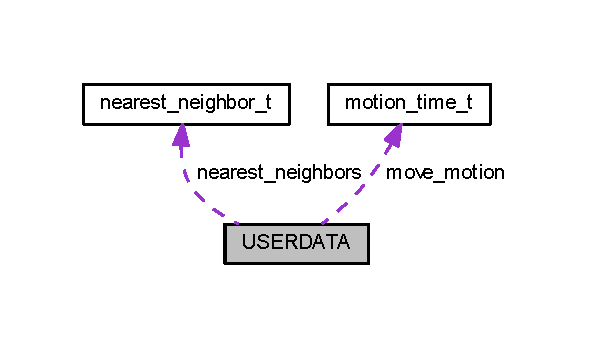
\includegraphics[width=284pt]{struct_u_s_e_r_d_a_t_a__coll__graph}
\end{center}
\end{figure}
\subsection*{Data Fields}
\begin{DoxyCompactItemize}
\item 
uint8\+\_\+t \hyperlink{struct_u_s_e_r_d_a_t_a_aa9d08e528bddaed76cb3ae2b3924e324}{my\+\_\+id}
\item 
uint8\+\_\+t \hyperlink{struct_u_s_e_r_d_a_t_a_acbbffd108b3e03fad207386744a5f5b7}{my\+\_\+right}
\item 
uint8\+\_\+t \hyperlink{struct_u_s_e_r_d_a_t_a_a7011a389bc4e0674c6d0d3dd1890c1a3}{my\+\_\+left}
\item 
message\+\_\+t \hyperlink{struct_u_s_e_r_d_a_t_a_a1bac7c8cafc9909ba9c076214a6b0c0b}{msg}
\item 
\hyperlink{ring_8h_a69b20b1a04c8e4cf3b72851b966259ec}{robot\+\_\+state} \hyperlink{struct_u_s_e_r_d_a_t_a_aadbb2fcd5b6edab38e3aa5aca6d92439}{state}
\item 
uint8\+\_\+t \hyperlink{struct_u_s_e_r_d_a_t_a_a5e6aae6522176125f4d02bba8ca5fe0c}{min\+\_\+id}
\item 
uint8\+\_\+t \hyperlink{struct_u_s_e_r_d_a_t_a_a05c940dbc220f5a723afd70071aebff8}{active}
\item 
uint8\+\_\+t \hyperlink{struct_u_s_e_r_d_a_t_a_ad87a0d3ed21e9d4050ce0eb138cb75b8}{num\+\_\+neighbors}
\item 
uint8\+\_\+t \hyperlink{struct_u_s_e_r_d_a_t_a_a83d1c1b9d1b27855cb1a36e755d73eb7}{message\+\_\+sent}
\item 
uint16\+\_\+t \hyperlink{struct_u_s_e_r_d_a_t_a_a95a543e244114d2368350d934a7392a6}{now}
\item 
uint16\+\_\+t \hyperlink{struct_u_s_e_r_d_a_t_a_aa0bb700e10f8de7a4a6a179e45ff78c6}{next\+\_\+share\+\_\+sending}
\item 
uint8\+\_\+t \hyperlink{struct_u_s_e_r_d_a_t_a_a01bba9e445a0f16707267c0ce23fb9b0}{cur\+\_\+motion}
\item 
uint8\+\_\+t \hyperlink{struct_u_s_e_r_d_a_t_a_a5cc036cf4f95c1f908b0253c67e6635d}{motion\+\_\+state}
\item 
uint8\+\_\+t \hyperlink{struct_u_s_e_r_d_a_t_a_a517ee3480ceae26e41c5807b94d1b3f3}{time\+\_\+active}
\item 
uint8\+\_\+t \hyperlink{struct_u_s_e_r_d_a_t_a_abf42309d619908c1318ec92fbd16cc6f}{move\+\_\+state}
\item 
\hyperlink{structnearest__neighbor__t}{nearest\+\_\+neighbor\+\_\+t} \hyperlink{struct_u_s_e_r_d_a_t_a_a7f78c5c44fd57c77fbc79f8f47913cac}{nearest\+\_\+neighbors} \mbox{[}\hyperlink{ring_8h_a7f85654336ae45adee0001ba8cdb8851}{M\+A\+X\+\_\+\+N\+U\+M\+\_\+\+N\+E\+I\+G\+H\+B\+O\+RS}\mbox{]}
\item 
\hyperlink{structmotion__time__t}{motion\+\_\+time\+\_\+t} \hyperlink{struct_u_s_e_r_d_a_t_a_a3398ac63ab67360828efdd1bef369245}{move\+\_\+motion} \mbox{[}3\mbox{]}
\item 
int8\+\_\+t \hyperlink{struct_u_s_e_r_d_a_t_a_ae0a633699328bd620301ffd914a44411}{send\+\_\+election}
\item 
int8\+\_\+t \hyperlink{struct_u_s_e_r_d_a_t_a_a4a20308ddbf35161cb24b5e5d9ca461e}{is\+\_\+leader}
\item 
uint8\+\_\+t \hyperlink{struct_u_s_e_r_d_a_t_a_a723f83660580bb0c28d7d3a92d02039e}{my\+\_\+leader}
\item 
uint8\+\_\+t \hyperlink{struct_u_s_e_r_d_a_t_a_a90d21fa503b626c00cdc8d94863d5877}{green}
\item 
uint8\+\_\+t \hyperlink{struct_u_s_e_r_d_a_t_a_ad47d918910aaa51c73160ac85999d09c}{red}
\item 
uint8\+\_\+t \hyperlink{struct_u_s_e_r_d_a_t_a_a287b397e90d7b995c81ff54e741f96b2}{blue}
\end{DoxyCompactItemize}


\subsection{Field Documentation}
\mbox{\Hypertarget{struct_u_s_e_r_d_a_t_a_a05c940dbc220f5a723afd70071aebff8}\label{struct_u_s_e_r_d_a_t_a_a05c940dbc220f5a723afd70071aebff8}} 
\index{U\+S\+E\+R\+D\+A\+TA@{U\+S\+E\+R\+D\+A\+TA}!active@{active}}
\index{active@{active}!U\+S\+E\+R\+D\+A\+TA@{U\+S\+E\+R\+D\+A\+TA}}
\subsubsection{\texorpdfstring{active}{active}}
{\footnotesize\ttfamily uint8\+\_\+t active}

\mbox{\Hypertarget{struct_u_s_e_r_d_a_t_a_a287b397e90d7b995c81ff54e741f96b2}\label{struct_u_s_e_r_d_a_t_a_a287b397e90d7b995c81ff54e741f96b2}} 
\index{U\+S\+E\+R\+D\+A\+TA@{U\+S\+E\+R\+D\+A\+TA}!blue@{blue}}
\index{blue@{blue}!U\+S\+E\+R\+D\+A\+TA@{U\+S\+E\+R\+D\+A\+TA}}
\subsubsection{\texorpdfstring{blue}{blue}}
{\footnotesize\ttfamily uint8\+\_\+t blue}

\mbox{\Hypertarget{struct_u_s_e_r_d_a_t_a_a01bba9e445a0f16707267c0ce23fb9b0}\label{struct_u_s_e_r_d_a_t_a_a01bba9e445a0f16707267c0ce23fb9b0}} 
\index{U\+S\+E\+R\+D\+A\+TA@{U\+S\+E\+R\+D\+A\+TA}!cur\+\_\+motion@{cur\+\_\+motion}}
\index{cur\+\_\+motion@{cur\+\_\+motion}!U\+S\+E\+R\+D\+A\+TA@{U\+S\+E\+R\+D\+A\+TA}}
\subsubsection{\texorpdfstring{cur\+\_\+motion}{cur\_motion}}
{\footnotesize\ttfamily uint8\+\_\+t cur\+\_\+motion}

\mbox{\Hypertarget{struct_u_s_e_r_d_a_t_a_a90d21fa503b626c00cdc8d94863d5877}\label{struct_u_s_e_r_d_a_t_a_a90d21fa503b626c00cdc8d94863d5877}} 
\index{U\+S\+E\+R\+D\+A\+TA@{U\+S\+E\+R\+D\+A\+TA}!green@{green}}
\index{green@{green}!U\+S\+E\+R\+D\+A\+TA@{U\+S\+E\+R\+D\+A\+TA}}
\subsubsection{\texorpdfstring{green}{green}}
{\footnotesize\ttfamily uint8\+\_\+t green}

\mbox{\Hypertarget{struct_u_s_e_r_d_a_t_a_a4a20308ddbf35161cb24b5e5d9ca461e}\label{struct_u_s_e_r_d_a_t_a_a4a20308ddbf35161cb24b5e5d9ca461e}} 
\index{U\+S\+E\+R\+D\+A\+TA@{U\+S\+E\+R\+D\+A\+TA}!is\+\_\+leader@{is\+\_\+leader}}
\index{is\+\_\+leader@{is\+\_\+leader}!U\+S\+E\+R\+D\+A\+TA@{U\+S\+E\+R\+D\+A\+TA}}
\subsubsection{\texorpdfstring{is\+\_\+leader}{is\_leader}}
{\footnotesize\ttfamily int8\+\_\+t is\+\_\+leader}

\mbox{\Hypertarget{struct_u_s_e_r_d_a_t_a_a83d1c1b9d1b27855cb1a36e755d73eb7}\label{struct_u_s_e_r_d_a_t_a_a83d1c1b9d1b27855cb1a36e755d73eb7}} 
\index{U\+S\+E\+R\+D\+A\+TA@{U\+S\+E\+R\+D\+A\+TA}!message\+\_\+sent@{message\+\_\+sent}}
\index{message\+\_\+sent@{message\+\_\+sent}!U\+S\+E\+R\+D\+A\+TA@{U\+S\+E\+R\+D\+A\+TA}}
\subsubsection{\texorpdfstring{message\+\_\+sent}{message\_sent}}
{\footnotesize\ttfamily uint8\+\_\+t message\+\_\+sent}

\mbox{\Hypertarget{struct_u_s_e_r_d_a_t_a_a5e6aae6522176125f4d02bba8ca5fe0c}\label{struct_u_s_e_r_d_a_t_a_a5e6aae6522176125f4d02bba8ca5fe0c}} 
\index{U\+S\+E\+R\+D\+A\+TA@{U\+S\+E\+R\+D\+A\+TA}!min\+\_\+id@{min\+\_\+id}}
\index{min\+\_\+id@{min\+\_\+id}!U\+S\+E\+R\+D\+A\+TA@{U\+S\+E\+R\+D\+A\+TA}}
\subsubsection{\texorpdfstring{min\+\_\+id}{min\_id}}
{\footnotesize\ttfamily uint8\+\_\+t min\+\_\+id}

\mbox{\Hypertarget{struct_u_s_e_r_d_a_t_a_a5cc036cf4f95c1f908b0253c67e6635d}\label{struct_u_s_e_r_d_a_t_a_a5cc036cf4f95c1f908b0253c67e6635d}} 
\index{U\+S\+E\+R\+D\+A\+TA@{U\+S\+E\+R\+D\+A\+TA}!motion\+\_\+state@{motion\+\_\+state}}
\index{motion\+\_\+state@{motion\+\_\+state}!U\+S\+E\+R\+D\+A\+TA@{U\+S\+E\+R\+D\+A\+TA}}
\subsubsection{\texorpdfstring{motion\+\_\+state}{motion\_state}}
{\footnotesize\ttfamily uint8\+\_\+t motion\+\_\+state}

\mbox{\Hypertarget{struct_u_s_e_r_d_a_t_a_a3398ac63ab67360828efdd1bef369245}\label{struct_u_s_e_r_d_a_t_a_a3398ac63ab67360828efdd1bef369245}} 
\index{U\+S\+E\+R\+D\+A\+TA@{U\+S\+E\+R\+D\+A\+TA}!move\+\_\+motion@{move\+\_\+motion}}
\index{move\+\_\+motion@{move\+\_\+motion}!U\+S\+E\+R\+D\+A\+TA@{U\+S\+E\+R\+D\+A\+TA}}
\subsubsection{\texorpdfstring{move\+\_\+motion}{move\_motion}}
{\footnotesize\ttfamily \hyperlink{structmotion__time__t}{motion\+\_\+time\+\_\+t} move\+\_\+motion\mbox{[}3\mbox{]}}

\mbox{\Hypertarget{struct_u_s_e_r_d_a_t_a_abf42309d619908c1318ec92fbd16cc6f}\label{struct_u_s_e_r_d_a_t_a_abf42309d619908c1318ec92fbd16cc6f}} 
\index{U\+S\+E\+R\+D\+A\+TA@{U\+S\+E\+R\+D\+A\+TA}!move\+\_\+state@{move\+\_\+state}}
\index{move\+\_\+state@{move\+\_\+state}!U\+S\+E\+R\+D\+A\+TA@{U\+S\+E\+R\+D\+A\+TA}}
\subsubsection{\texorpdfstring{move\+\_\+state}{move\_state}}
{\footnotesize\ttfamily uint8\+\_\+t move\+\_\+state}

\mbox{\Hypertarget{struct_u_s_e_r_d_a_t_a_a1bac7c8cafc9909ba9c076214a6b0c0b}\label{struct_u_s_e_r_d_a_t_a_a1bac7c8cafc9909ba9c076214a6b0c0b}} 
\index{U\+S\+E\+R\+D\+A\+TA@{U\+S\+E\+R\+D\+A\+TA}!msg@{msg}}
\index{msg@{msg}!U\+S\+E\+R\+D\+A\+TA@{U\+S\+E\+R\+D\+A\+TA}}
\subsubsection{\texorpdfstring{msg}{msg}}
{\footnotesize\ttfamily message\+\_\+t msg}

\mbox{\Hypertarget{struct_u_s_e_r_d_a_t_a_aa9d08e528bddaed76cb3ae2b3924e324}\label{struct_u_s_e_r_d_a_t_a_aa9d08e528bddaed76cb3ae2b3924e324}} 
\index{U\+S\+E\+R\+D\+A\+TA@{U\+S\+E\+R\+D\+A\+TA}!my\+\_\+id@{my\+\_\+id}}
\index{my\+\_\+id@{my\+\_\+id}!U\+S\+E\+R\+D\+A\+TA@{U\+S\+E\+R\+D\+A\+TA}}
\subsubsection{\texorpdfstring{my\+\_\+id}{my\_id}}
{\footnotesize\ttfamily uint8\+\_\+t my\+\_\+id}

\mbox{\Hypertarget{struct_u_s_e_r_d_a_t_a_a723f83660580bb0c28d7d3a92d02039e}\label{struct_u_s_e_r_d_a_t_a_a723f83660580bb0c28d7d3a92d02039e}} 
\index{U\+S\+E\+R\+D\+A\+TA@{U\+S\+E\+R\+D\+A\+TA}!my\+\_\+leader@{my\+\_\+leader}}
\index{my\+\_\+leader@{my\+\_\+leader}!U\+S\+E\+R\+D\+A\+TA@{U\+S\+E\+R\+D\+A\+TA}}
\subsubsection{\texorpdfstring{my\+\_\+leader}{my\_leader}}
{\footnotesize\ttfamily uint8\+\_\+t my\+\_\+leader}

\mbox{\Hypertarget{struct_u_s_e_r_d_a_t_a_a7011a389bc4e0674c6d0d3dd1890c1a3}\label{struct_u_s_e_r_d_a_t_a_a7011a389bc4e0674c6d0d3dd1890c1a3}} 
\index{U\+S\+E\+R\+D\+A\+TA@{U\+S\+E\+R\+D\+A\+TA}!my\+\_\+left@{my\+\_\+left}}
\index{my\+\_\+left@{my\+\_\+left}!U\+S\+E\+R\+D\+A\+TA@{U\+S\+E\+R\+D\+A\+TA}}
\subsubsection{\texorpdfstring{my\+\_\+left}{my\_left}}
{\footnotesize\ttfamily uint8\+\_\+t my\+\_\+left}

\mbox{\Hypertarget{struct_u_s_e_r_d_a_t_a_acbbffd108b3e03fad207386744a5f5b7}\label{struct_u_s_e_r_d_a_t_a_acbbffd108b3e03fad207386744a5f5b7}} 
\index{U\+S\+E\+R\+D\+A\+TA@{U\+S\+E\+R\+D\+A\+TA}!my\+\_\+right@{my\+\_\+right}}
\index{my\+\_\+right@{my\+\_\+right}!U\+S\+E\+R\+D\+A\+TA@{U\+S\+E\+R\+D\+A\+TA}}
\subsubsection{\texorpdfstring{my\+\_\+right}{my\_right}}
{\footnotesize\ttfamily uint8\+\_\+t my\+\_\+right}

\mbox{\Hypertarget{struct_u_s_e_r_d_a_t_a_a7f78c5c44fd57c77fbc79f8f47913cac}\label{struct_u_s_e_r_d_a_t_a_a7f78c5c44fd57c77fbc79f8f47913cac}} 
\index{U\+S\+E\+R\+D\+A\+TA@{U\+S\+E\+R\+D\+A\+TA}!nearest\+\_\+neighbors@{nearest\+\_\+neighbors}}
\index{nearest\+\_\+neighbors@{nearest\+\_\+neighbors}!U\+S\+E\+R\+D\+A\+TA@{U\+S\+E\+R\+D\+A\+TA}}
\subsubsection{\texorpdfstring{nearest\+\_\+neighbors}{nearest\_neighbors}}
{\footnotesize\ttfamily \hyperlink{structnearest__neighbor__t}{nearest\+\_\+neighbor\+\_\+t} nearest\+\_\+neighbors\mbox{[}\hyperlink{ring_8h_a7f85654336ae45adee0001ba8cdb8851}{M\+A\+X\+\_\+\+N\+U\+M\+\_\+\+N\+E\+I\+G\+H\+B\+O\+RS}\mbox{]}}

\mbox{\Hypertarget{struct_u_s_e_r_d_a_t_a_aa0bb700e10f8de7a4a6a179e45ff78c6}\label{struct_u_s_e_r_d_a_t_a_aa0bb700e10f8de7a4a6a179e45ff78c6}} 
\index{U\+S\+E\+R\+D\+A\+TA@{U\+S\+E\+R\+D\+A\+TA}!next\+\_\+share\+\_\+sending@{next\+\_\+share\+\_\+sending}}
\index{next\+\_\+share\+\_\+sending@{next\+\_\+share\+\_\+sending}!U\+S\+E\+R\+D\+A\+TA@{U\+S\+E\+R\+D\+A\+TA}}
\subsubsection{\texorpdfstring{next\+\_\+share\+\_\+sending}{next\_share\_sending}}
{\footnotesize\ttfamily uint16\+\_\+t next\+\_\+share\+\_\+sending}

\mbox{\Hypertarget{struct_u_s_e_r_d_a_t_a_a95a543e244114d2368350d934a7392a6}\label{struct_u_s_e_r_d_a_t_a_a95a543e244114d2368350d934a7392a6}} 
\index{U\+S\+E\+R\+D\+A\+TA@{U\+S\+E\+R\+D\+A\+TA}!now@{now}}
\index{now@{now}!U\+S\+E\+R\+D\+A\+TA@{U\+S\+E\+R\+D\+A\+TA}}
\subsubsection{\texorpdfstring{now}{now}}
{\footnotesize\ttfamily uint16\+\_\+t now}

\mbox{\Hypertarget{struct_u_s_e_r_d_a_t_a_ad87a0d3ed21e9d4050ce0eb138cb75b8}\label{struct_u_s_e_r_d_a_t_a_ad87a0d3ed21e9d4050ce0eb138cb75b8}} 
\index{U\+S\+E\+R\+D\+A\+TA@{U\+S\+E\+R\+D\+A\+TA}!num\+\_\+neighbors@{num\+\_\+neighbors}}
\index{num\+\_\+neighbors@{num\+\_\+neighbors}!U\+S\+E\+R\+D\+A\+TA@{U\+S\+E\+R\+D\+A\+TA}}
\subsubsection{\texorpdfstring{num\+\_\+neighbors}{num\_neighbors}}
{\footnotesize\ttfamily uint8\+\_\+t num\+\_\+neighbors}

\mbox{\Hypertarget{struct_u_s_e_r_d_a_t_a_ad47d918910aaa51c73160ac85999d09c}\label{struct_u_s_e_r_d_a_t_a_ad47d918910aaa51c73160ac85999d09c}} 
\index{U\+S\+E\+R\+D\+A\+TA@{U\+S\+E\+R\+D\+A\+TA}!red@{red}}
\index{red@{red}!U\+S\+E\+R\+D\+A\+TA@{U\+S\+E\+R\+D\+A\+TA}}
\subsubsection{\texorpdfstring{red}{red}}
{\footnotesize\ttfamily uint8\+\_\+t red}

\mbox{\Hypertarget{struct_u_s_e_r_d_a_t_a_ae0a633699328bd620301ffd914a44411}\label{struct_u_s_e_r_d_a_t_a_ae0a633699328bd620301ffd914a44411}} 
\index{U\+S\+E\+R\+D\+A\+TA@{U\+S\+E\+R\+D\+A\+TA}!send\+\_\+election@{send\+\_\+election}}
\index{send\+\_\+election@{send\+\_\+election}!U\+S\+E\+R\+D\+A\+TA@{U\+S\+E\+R\+D\+A\+TA}}
\subsubsection{\texorpdfstring{send\+\_\+election}{send\_election}}
{\footnotesize\ttfamily int8\+\_\+t send\+\_\+election}

\mbox{\Hypertarget{struct_u_s_e_r_d_a_t_a_aadbb2fcd5b6edab38e3aa5aca6d92439}\label{struct_u_s_e_r_d_a_t_a_aadbb2fcd5b6edab38e3aa5aca6d92439}} 
\index{U\+S\+E\+R\+D\+A\+TA@{U\+S\+E\+R\+D\+A\+TA}!state@{state}}
\index{state@{state}!U\+S\+E\+R\+D\+A\+TA@{U\+S\+E\+R\+D\+A\+TA}}
\subsubsection{\texorpdfstring{state}{state}}
{\footnotesize\ttfamily \hyperlink{ring_8h_a69b20b1a04c8e4cf3b72851b966259ec}{robot\+\_\+state} state}

\mbox{\Hypertarget{struct_u_s_e_r_d_a_t_a_a517ee3480ceae26e41c5807b94d1b3f3}\label{struct_u_s_e_r_d_a_t_a_a517ee3480ceae26e41c5807b94d1b3f3}} 
\index{U\+S\+E\+R\+D\+A\+TA@{U\+S\+E\+R\+D\+A\+TA}!time\+\_\+active@{time\+\_\+active}}
\index{time\+\_\+active@{time\+\_\+active}!U\+S\+E\+R\+D\+A\+TA@{U\+S\+E\+R\+D\+A\+TA}}
\subsubsection{\texorpdfstring{time\+\_\+active}{time\_active}}
{\footnotesize\ttfamily uint8\+\_\+t time\+\_\+active}



The documentation for this struct was generated from the following file\+:\begin{DoxyCompactItemize}
\item 
\hyperlink{ring_8h}{ring.\+h}\end{DoxyCompactItemize}

\chapter{File Documentation}
\hypertarget{ring_8c}{}\section{ring.\+c File Reference}
\label{ring_8c}\index{ring.\+c@{ring.\+c}}
{\ttfamily \#include $<$math.\+h$>$}\newline
{\ttfamily \#include $<$kilombo.\+h$>$}\newline
{\ttfamily \#include $<$stdio.\+h$>$}\newline
{\ttfamily \#include \char`\"{}ring.\+h\char`\"{}}\newline
Include dependency graph for ring.\+c\+:\nopagebreak
\begin{figure}[H]
\begin{center}
\leavevmode
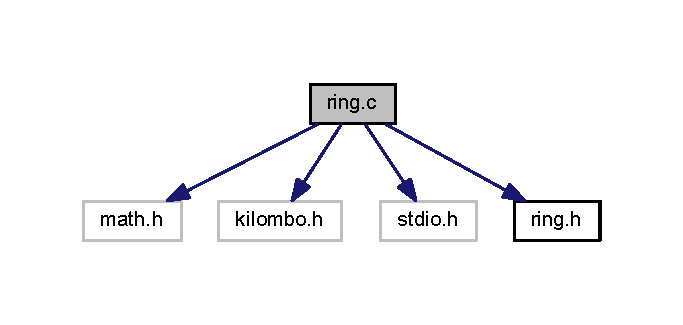
\includegraphics[width=328pt]{ring_8c__incl}
\end{center}
\end{figure}
\subsection*{Functions}
\begin{DoxyCompactItemize}
\item 
void \hyperlink{ring_8c_a540b8ce2367b2cf4b32c8b8c7e9642fc}{smooth\+\_\+set\+\_\+motors} (uint8\+\_\+t ccw, uint8\+\_\+t cw)
\item 
void \hyperlink{ring_8c_a88524e838112e1905cc3f74b0735ae71}{set\+\_\+motion} (\hyperlink{ring_8h_af714dce6622a529fd1e432cb0dbfe0a1}{motion\+\_\+t} new\+\_\+motion)
\item 
char \hyperlink{ring_8c_a764ba1034860f888b777fdf475143667}{in\+\_\+interval} (uint8\+\_\+t distance)
\item 
char \hyperlink{ring_8c_a77db9a24f35da1c9278ccd2d15720552}{is\+\_\+stabilized} ()
\item 
uint8\+\_\+t \hyperlink{ring_8c_a421bd0c8e972c872a4c101c7fe2776db}{exists\+\_\+nearest\+\_\+neighbor} (uint8\+\_\+t id)
\item 
uint8\+\_\+t \hyperlink{ring_8c_acc148f4ab3c9d5f09b3db2a3077b3fc1}{are\+\_\+all\+\_\+cooperative} ()
\item 
uint8\+\_\+t \hyperlink{ring_8c_af19fc3162e19356dfdd8d2d04fb98ad9}{get\+\_\+nearest\+\_\+two\+\_\+neighbors} ()
\item 
void \hyperlink{ring_8c_ad8d6e8bd005b92febac972bac5171128}{recv\+\_\+sharing} (uint8\+\_\+t $\ast$payload, uint8\+\_\+t distance)
\item 
void \hyperlink{ring_8c_a27b20f1b26960043194f20584b81f3c9}{recv\+\_\+joining} (uint8\+\_\+t $\ast$payload)
\item 
void \hyperlink{ring_8c_ac178becefc5a6cb069d7204976ae4506}{recv\+\_\+election} (uint8\+\_\+t $\ast$payload)
\item 
void \hyperlink{ring_8c_a41166d26230bdddde589f3ab36a422b6}{message\+\_\+rx} (message\+\_\+t $\ast$m, distance\+\_\+measurement\+\_\+t $\ast$d)
\item 
void \hyperlink{ring_8c_ad1b5e8bdcafee199c2a5e0f255ac6585}{prepare\+\_\+message} (uint8\+\_\+t m, uint8\+\_\+t receiver)
\item 
void \hyperlink{ring_8c_a1695dcc0c6a920317d739886e3266093}{send\+\_\+joining} ()
\item 
void \hyperlink{ring_8c_a95a8f45823e9116b153d0b1f7eaa6201}{send\+\_\+sharing} ()
\item 
void \hyperlink{ring_8c_ab9082108a5add8649dfe4d65c7d7b676}{send\+\_\+election} ()
\item 
void \hyperlink{ring_8c_a34f4768b59989ab2a1fa2e480b7b3f33}{move} (uint8\+\_\+t tick)
\item 
void \hyperlink{ring_8c_afe461d27b9c48d5921c00d521181f12f}{loop} ()
\item 
message\+\_\+t $\ast$ \hyperlink{ring_8c_a7fe98b6e71da81f72143305f649beb63}{message\+\_\+tx} ()
\item 
void \hyperlink{ring_8c_a0f57ca4676befec475a590c8b8d78d8e}{message\+\_\+tx\+\_\+success} ()
\item 
void \hyperlink{ring_8c_a4fc01d736fe50cf5b977f755b675f11d}{setup} ()
\item 
int \hyperlink{ring_8c_ae66f6b31b5ad750f1fe042a706a4e3d4}{main} ()
\end{DoxyCompactItemize}


\subsection{Function Documentation}
\mbox{\Hypertarget{ring_8c_acc148f4ab3c9d5f09b3db2a3077b3fc1}\label{ring_8c_acc148f4ab3c9d5f09b3db2a3077b3fc1}} 
\index{ring.\+c@{ring.\+c}!are\+\_\+all\+\_\+cooperative@{are\+\_\+all\+\_\+cooperative}}
\index{are\+\_\+all\+\_\+cooperative@{are\+\_\+all\+\_\+cooperative}!ring.\+c@{ring.\+c}}
\subsubsection{\texorpdfstring{are\+\_\+all\+\_\+cooperative()}{are\_all\_cooperative()}}
{\footnotesize\ttfamily uint8\+\_\+t are\+\_\+all\+\_\+cooperative (\begin{DoxyParamCaption}{ }\end{DoxyParamCaption})}

Helper function to make sure the nodes are connecting \mbox{\Hypertarget{ring_8c_a421bd0c8e972c872a4c101c7fe2776db}\label{ring_8c_a421bd0c8e972c872a4c101c7fe2776db}} 
\index{ring.\+c@{ring.\+c}!exists\+\_\+nearest\+\_\+neighbor@{exists\+\_\+nearest\+\_\+neighbor}}
\index{exists\+\_\+nearest\+\_\+neighbor@{exists\+\_\+nearest\+\_\+neighbor}!ring.\+c@{ring.\+c}}
\subsubsection{\texorpdfstring{exists\+\_\+nearest\+\_\+neighbor()}{exists\_nearest\_neighbor()}}
{\footnotesize\ttfamily uint8\+\_\+t exists\+\_\+nearest\+\_\+neighbor (\begin{DoxyParamCaption}\item[{uint8\+\_\+t}]{id }\end{DoxyParamCaption})}

Helper function for setting distance


\begin{DoxyParams}{Parameters}
{\em id} & Integer that contains the distance for the motor \\
\hline
\end{DoxyParams}
\mbox{\Hypertarget{ring_8c_af19fc3162e19356dfdd8d2d04fb98ad9}\label{ring_8c_af19fc3162e19356dfdd8d2d04fb98ad9}} 
\index{ring.\+c@{ring.\+c}!get\+\_\+nearest\+\_\+two\+\_\+neighbors@{get\+\_\+nearest\+\_\+two\+\_\+neighbors}}
\index{get\+\_\+nearest\+\_\+two\+\_\+neighbors@{get\+\_\+nearest\+\_\+two\+\_\+neighbors}!ring.\+c@{ring.\+c}}
\subsubsection{\texorpdfstring{get\+\_\+nearest\+\_\+two\+\_\+neighbors()}{get\_nearest\_two\_neighbors()}}
{\footnotesize\ttfamily uint8\+\_\+t get\+\_\+nearest\+\_\+two\+\_\+neighbors (\begin{DoxyParamCaption}{ }\end{DoxyParamCaption})}

Function that obtains the nearest two node neighbors for a particular node. \mbox{\Hypertarget{ring_8c_a764ba1034860f888b777fdf475143667}\label{ring_8c_a764ba1034860f888b777fdf475143667}} 
\index{ring.\+c@{ring.\+c}!in\+\_\+interval@{in\+\_\+interval}}
\index{in\+\_\+interval@{in\+\_\+interval}!ring.\+c@{ring.\+c}}
\subsubsection{\texorpdfstring{in\+\_\+interval()}{in\_interval()}}
{\footnotesize\ttfamily char in\+\_\+interval (\begin{DoxyParamCaption}\item[{uint8\+\_\+t}]{distance }\end{DoxyParamCaption})}

Helper function for setting distance


\begin{DoxyParams}{Parameters}
{\em distance} & Integer that contains the distance for the motor \\
\hline
\end{DoxyParams}
\mbox{\Hypertarget{ring_8c_a77db9a24f35da1c9278ccd2d15720552}\label{ring_8c_a77db9a24f35da1c9278ccd2d15720552}} 
\index{ring.\+c@{ring.\+c}!is\+\_\+stabilized@{is\+\_\+stabilized}}
\index{is\+\_\+stabilized@{is\+\_\+stabilized}!ring.\+c@{ring.\+c}}
\subsubsection{\texorpdfstring{is\+\_\+stabilized()}{is\_stabilized()}}
{\footnotesize\ttfamily char is\+\_\+stabilized (\begin{DoxyParamCaption}{ }\end{DoxyParamCaption})}

Helper function to check the node to see if it\textquotesingle{}s stablized \mbox{\Hypertarget{ring_8c_afe461d27b9c48d5921c00d521181f12f}\label{ring_8c_afe461d27b9c48d5921c00d521181f12f}} 
\index{ring.\+c@{ring.\+c}!loop@{loop}}
\index{loop@{loop}!ring.\+c@{ring.\+c}}
\subsubsection{\texorpdfstring{loop()}{loop()}}
{\footnotesize\ttfamily void loop (\begin{DoxyParamCaption}{ }\end{DoxyParamCaption})}

Helper function for the loop of the program \mbox{\Hypertarget{ring_8c_ae66f6b31b5ad750f1fe042a706a4e3d4}\label{ring_8c_ae66f6b31b5ad750f1fe042a706a4e3d4}} 
\index{ring.\+c@{ring.\+c}!main@{main}}
\index{main@{main}!ring.\+c@{ring.\+c}}
\subsubsection{\texorpdfstring{main()}{main()}}
{\footnotesize\ttfamily int main (\begin{DoxyParamCaption}{ }\end{DoxyParamCaption})}

\mbox{\Hypertarget{ring_8c_a41166d26230bdddde589f3ab36a422b6}\label{ring_8c_a41166d26230bdddde589f3ab36a422b6}} 
\index{ring.\+c@{ring.\+c}!message\+\_\+rx@{message\+\_\+rx}}
\index{message\+\_\+rx@{message\+\_\+rx}!ring.\+c@{ring.\+c}}
\subsubsection{\texorpdfstring{message\+\_\+rx()}{message\_rx()}}
{\footnotesize\ttfamily void message\+\_\+rx (\begin{DoxyParamCaption}\item[{message\+\_\+t $\ast$}]{m,  }\item[{distance\+\_\+measurement\+\_\+t $\ast$}]{d }\end{DoxyParamCaption})}

Helper function for sending the message


\begin{DoxyParams}{Parameters}
{\em m} & pointer that contains the message for the motor \\
\hline
{\em d} & pointer that contains the distance of the motor \\
\hline
\end{DoxyParams}
\mbox{\Hypertarget{ring_8c_a7fe98b6e71da81f72143305f649beb63}\label{ring_8c_a7fe98b6e71da81f72143305f649beb63}} 
\index{ring.\+c@{ring.\+c}!message\+\_\+tx@{message\+\_\+tx}}
\index{message\+\_\+tx@{message\+\_\+tx}!ring.\+c@{ring.\+c}}
\subsubsection{\texorpdfstring{message\+\_\+tx()}{message\_tx()}}
{\footnotesize\ttfamily message\+\_\+t$\ast$ message\+\_\+tx (\begin{DoxyParamCaption}{ }\end{DoxyParamCaption})}

function for the message \mbox{\Hypertarget{ring_8c_a0f57ca4676befec475a590c8b8d78d8e}\label{ring_8c_a0f57ca4676befec475a590c8b8d78d8e}} 
\index{ring.\+c@{ring.\+c}!message\+\_\+tx\+\_\+success@{message\+\_\+tx\+\_\+success}}
\index{message\+\_\+tx\+\_\+success@{message\+\_\+tx\+\_\+success}!ring.\+c@{ring.\+c}}
\subsubsection{\texorpdfstring{message\+\_\+tx\+\_\+success()}{message\_tx\_success()}}
{\footnotesize\ttfamily void message\+\_\+tx\+\_\+success (\begin{DoxyParamCaption}{ }\end{DoxyParamCaption})}

Determines whether or not the message was successfully sent \mbox{\Hypertarget{ring_8c_a34f4768b59989ab2a1fa2e480b7b3f33}\label{ring_8c_a34f4768b59989ab2a1fa2e480b7b3f33}} 
\index{ring.\+c@{ring.\+c}!move@{move}}
\index{move@{move}!ring.\+c@{ring.\+c}}
\subsubsection{\texorpdfstring{move()}{move()}}
{\footnotesize\ttfamily void move (\begin{DoxyParamCaption}\item[{uint8\+\_\+t}]{tick }\end{DoxyParamCaption})}

Helper function for setting distance


\begin{DoxyParams}{Parameters}
{\em tick} & Integer that contains the ticks for the motor \\
\hline
\end{DoxyParams}
\mbox{\Hypertarget{ring_8c_ad1b5e8bdcafee199c2a5e0f255ac6585}\label{ring_8c_ad1b5e8bdcafee199c2a5e0f255ac6585}} 
\index{ring.\+c@{ring.\+c}!prepare\+\_\+message@{prepare\+\_\+message}}
\index{prepare\+\_\+message@{prepare\+\_\+message}!ring.\+c@{ring.\+c}}
\subsubsection{\texorpdfstring{prepare\+\_\+message()}{prepare\_message()}}
{\footnotesize\ttfamily void prepare\+\_\+message (\begin{DoxyParamCaption}\item[{uint8\+\_\+t}]{m,  }\item[{uint8\+\_\+t}]{receiver }\end{DoxyParamCaption})}

Function for preparing the message for the node to be sent


\begin{DoxyParams}{Parameters}
{\em m} & Integer that contains the message for the motor \\
\hline
{\em receiver} & Integer that contains the ID of the motor to be receiving the message \\
\hline
\end{DoxyParams}
\mbox{\Hypertarget{ring_8c_ac178becefc5a6cb069d7204976ae4506}\label{ring_8c_ac178becefc5a6cb069d7204976ae4506}} 
\index{ring.\+c@{ring.\+c}!recv\+\_\+election@{recv\+\_\+election}}
\index{recv\+\_\+election@{recv\+\_\+election}!ring.\+c@{ring.\+c}}
\subsubsection{\texorpdfstring{recv\+\_\+election()}{recv\_election()}}
{\footnotesize\ttfamily void recv\+\_\+election (\begin{DoxyParamCaption}\item[{uint8\+\_\+t $\ast$}]{payload }\end{DoxyParamCaption})}

Helper function to help the receiving node can be elected the leader of the group


\begin{DoxyParams}{Parameters}
{\em payload} & Integer that contains the payload of the motor \\
\hline
\end{DoxyParams}
v = mydata-\/$>$my\+\_\+id w = payload\mbox{[}leader\mbox{]} m = min\+\_\+id\mbox{\Hypertarget{ring_8c_a27b20f1b26960043194f20584b81f3c9}\label{ring_8c_a27b20f1b26960043194f20584b81f3c9}} 
\index{ring.\+c@{ring.\+c}!recv\+\_\+joining@{recv\+\_\+joining}}
\index{recv\+\_\+joining@{recv\+\_\+joining}!ring.\+c@{ring.\+c}}
\subsubsection{\texorpdfstring{recv\+\_\+joining()}{recv\_joining()}}
{\footnotesize\ttfamily void recv\+\_\+joining (\begin{DoxyParamCaption}\item[{uint8\+\_\+t $\ast$}]{payload }\end{DoxyParamCaption})}

Helper function for making sure the receiving node is able to join the group


\begin{DoxyParams}{Parameters}
{\em payload} & Integer that contains the payload of the motor \\
\hline
\end{DoxyParams}
\mbox{\Hypertarget{ring_8c_ad8d6e8bd005b92febac972bac5171128}\label{ring_8c_ad8d6e8bd005b92febac972bac5171128}} 
\index{ring.\+c@{ring.\+c}!recv\+\_\+sharing@{recv\+\_\+sharing}}
\index{recv\+\_\+sharing@{recv\+\_\+sharing}!ring.\+c@{ring.\+c}}
\subsubsection{\texorpdfstring{recv\+\_\+sharing()}{recv\_sharing()}}
{\footnotesize\ttfamily void recv\+\_\+sharing (\begin{DoxyParamCaption}\item[{uint8\+\_\+t $\ast$}]{payload,  }\item[{uint8\+\_\+t}]{distance }\end{DoxyParamCaption})}

Helper function for making sure the receiving node obtains the message


\begin{DoxyParams}{Parameters}
{\em distance} & Integer that contains the distance for the motor \\
\hline
{\em payload} & Integer that contains the payload of the motor \\
\hline
\end{DoxyParams}
\mbox{\Hypertarget{ring_8c_ab9082108a5add8649dfe4d65c7d7b676}\label{ring_8c_ab9082108a5add8649dfe4d65c7d7b676}} 
\index{ring.\+c@{ring.\+c}!send\+\_\+election@{send\+\_\+election}}
\index{send\+\_\+election@{send\+\_\+election}!ring.\+c@{ring.\+c}}
\subsubsection{\texorpdfstring{send\+\_\+election()}{send\_election()}}
{\footnotesize\ttfamily void send\+\_\+election (\begin{DoxyParamCaption}{ }\end{DoxyParamCaption})}

Helper function for the node to send an election message \mbox{\Hypertarget{ring_8c_a1695dcc0c6a920317d739886e3266093}\label{ring_8c_a1695dcc0c6a920317d739886e3266093}} 
\index{ring.\+c@{ring.\+c}!send\+\_\+joining@{send\+\_\+joining}}
\index{send\+\_\+joining@{send\+\_\+joining}!ring.\+c@{ring.\+c}}
\subsubsection{\texorpdfstring{send\+\_\+joining()}{send\_joining()}}
{\footnotesize\ttfamily void send\+\_\+joining (\begin{DoxyParamCaption}{ }\end{DoxyParamCaption})}

Helper function for the initial node to join the group \mbox{\Hypertarget{ring_8c_a95a8f45823e9116b153d0b1f7eaa6201}\label{ring_8c_a95a8f45823e9116b153d0b1f7eaa6201}} 
\index{ring.\+c@{ring.\+c}!send\+\_\+sharing@{send\+\_\+sharing}}
\index{send\+\_\+sharing@{send\+\_\+sharing}!ring.\+c@{ring.\+c}}
\subsubsection{\texorpdfstring{send\+\_\+sharing()}{send\_sharing()}}
{\footnotesize\ttfamily void send\+\_\+sharing (\begin{DoxyParamCaption}{ }\end{DoxyParamCaption})}

Helper function for the initial node to share the message to the receiving node \mbox{\Hypertarget{ring_8c_a88524e838112e1905cc3f74b0735ae71}\label{ring_8c_a88524e838112e1905cc3f74b0735ae71}} 
\index{ring.\+c@{ring.\+c}!set\+\_\+motion@{set\+\_\+motion}}
\index{set\+\_\+motion@{set\+\_\+motion}!ring.\+c@{ring.\+c}}
\subsubsection{\texorpdfstring{set\+\_\+motion()}{set\_motion()}}
{\footnotesize\ttfamily void set\+\_\+motion (\begin{DoxyParamCaption}\item[{\hyperlink{ring_8h_af714dce6622a529fd1e432cb0dbfe0a1}{motion\+\_\+t}}]{new\+\_\+motion }\end{DoxyParamCaption})}

Helper function that sets the motion of the motor


\begin{DoxyParams}{Parameters}
{\em new\+\_\+motion} & Determines where the motor moves \\
\hline
\end{DoxyParams}
\mbox{\Hypertarget{ring_8c_a4fc01d736fe50cf5b977f755b675f11d}\label{ring_8c_a4fc01d736fe50cf5b977f755b675f11d}} 
\index{ring.\+c@{ring.\+c}!setup@{setup}}
\index{setup@{setup}!ring.\+c@{ring.\+c}}
\subsubsection{\texorpdfstring{setup()}{setup()}}
{\footnotesize\ttfamily void setup (\begin{DoxyParamCaption}{ }\end{DoxyParamCaption})}

Sets up the program \mbox{\Hypertarget{ring_8c_a540b8ce2367b2cf4b32c8b8c7e9642fc}\label{ring_8c_a540b8ce2367b2cf4b32c8b8c7e9642fc}} 
\index{ring.\+c@{ring.\+c}!smooth\+\_\+set\+\_\+motors@{smooth\+\_\+set\+\_\+motors}}
\index{smooth\+\_\+set\+\_\+motors@{smooth\+\_\+set\+\_\+motors}!ring.\+c@{ring.\+c}}
\subsubsection{\texorpdfstring{smooth\+\_\+set\+\_\+motors()}{smooth\_set\_motors()}}
{\footnotesize\ttfamily void smooth\+\_\+set\+\_\+motors (\begin{DoxyParamCaption}\item[{uint8\+\_\+t}]{ccw,  }\item[{uint8\+\_\+t}]{cw }\end{DoxyParamCaption})}

Helper function for setting motor speed smoothly


\begin{DoxyParams}{Parameters}
{\em ccw} & Integer that sets motors as counter-\/clockwise \\
\hline
{\em cw} & Integer that sets motors as clockwise \\
\hline
\end{DoxyParams}

\hypertarget{ring_8h}{}\section{ring.\+h File Reference}
\label{ring_8h}\index{ring.\+h@{ring.\+h}}
This graph shows which files directly or indirectly include this file\+:\nopagebreak
\begin{figure}[H]
\begin{center}
\leavevmode
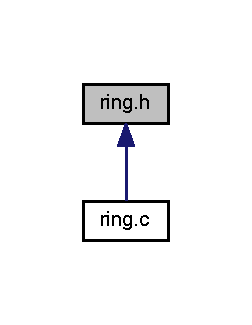
\includegraphics[width=121pt]{ring_8h__dep__incl}
\end{center}
\end{figure}
\subsection*{Data Structures}
\begin{DoxyCompactItemize}
\item 
struct \hyperlink{structnearest__neighbor__t}{nearest\+\_\+neighbor\+\_\+t}
\item 
struct \hyperlink{structmotion__time__t}{motion\+\_\+time\+\_\+t}
\item 
struct \hyperlink{struct_u_s_e_r_d_a_t_a}{U\+S\+E\+R\+D\+A\+TA}
\end{DoxyCompactItemize}
\subsection*{Macros}
\begin{DoxyCompactItemize}
\item 
\#define \hyperlink{ring_8h_a7f85654336ae45adee0001ba8cdb8851}{M\+A\+X\+\_\+\+N\+U\+M\+\_\+\+N\+E\+I\+G\+H\+B\+O\+RS}~10
\item 
\#define \hyperlink{ring_8h_a8eb91fb063c5d18e88bb6c778f7de643}{S\+H\+A\+R\+I\+N\+G\+\_\+\+T\+I\+ME}~20
\item 
\#define \hyperlink{ring_8h_a0c719c414608ef14852670b063876c07}{M\+SG}~0
\item 
\#define \hyperlink{ring_8h_a77ceac8d6af195fe72f95f6afd87c45e}{ID}~1
\item 
\#define \hyperlink{ring_8h_af23fdd273a208806b49daf7499e0d9f2}{R\+I\+G\+H\+T\+\_\+\+ID}~2
\item 
\#define \hyperlink{ring_8h_add101440435d6b76ecf18896c9eefc80}{L\+E\+F\+T\+\_\+\+ID}~3
\item 
\#define \hyperlink{ring_8h_aacd2cf60f504e45efada9aec028ee3cd}{S\+T\+A\+TE}~4
\item 
\#define \hyperlink{ring_8h_a455948b8bd5f5ce920899ae1013c4b4c}{R\+E\+C\+E\+I\+V\+ER}~5
\item 
\#define \hyperlink{ring_8h_afe3a5d0081166bd5e1d8c9ea00db83e5}{S\+E\+N\+D\+ER}~6
\item 
\#define \hyperlink{ring_8h_abfa4129c01696b7e625c9f18fc2dfd6d}{L\+E\+A\+D\+ER}~7
\item 
\#define \hyperlink{ring_8h_a3a6d3cd70078e6046471ec528a09cd19}{A\+C\+T\+I\+VE}~0
\item 
\#define \hyperlink{ring_8h_ae71449b1cc6e6250b91f539153a7a0d3}{M\+\_\+\+PI}~3.\+141592653589793238462643383279502884197169399375105820974944
\end{DoxyCompactItemize}
\subsection*{Enumerations}
\begin{DoxyCompactItemize}
\item 
enum \hyperlink{ring_8h_a4e0a9e26bf11796d8ca091cb6b3ce470}{message\+\_\+type} \{ \newline
\hyperlink{ring_8h_a4e0a9e26bf11796d8ca091cb6b3ce470a2e269dfbf70bb56eddcf95b39bf94d2e}{N\+U\+L\+L\+\_\+\+M\+SG}, 
\hyperlink{ring_8h_a4e0a9e26bf11796d8ca091cb6b3ce470a3754861e8c074fb088a2ed4f64786268}{S\+H\+A\+RE}, 
\hyperlink{ring_8h_a4e0a9e26bf11796d8ca091cb6b3ce470a4925a399dab94b9b58f6d1b5cd246af7}{J\+O\+IN}, 
\hyperlink{ring_8h_a4e0a9e26bf11796d8ca091cb6b3ce470ae09e07839103de682cb13fa773793fc0}{L\+E\+A\+VE}, 
\newline
\hyperlink{ring_8h_a4e0a9e26bf11796d8ca091cb6b3ce470adca3ea7fa09ef8a260d98e3f62b72636}{E\+L\+E\+C\+T\+I\+ON}
 \}
\item 
enum \hyperlink{ring_8h_a69b20b1a04c8e4cf3b72851b966259ec}{robot\+\_\+state} \{ \hyperlink{ring_8h_a69b20b1a04c8e4cf3b72851b966259eca15984d1e548813ca0e54895a2322b54b}{A\+U\+T\+O\+N\+O\+M\+O\+US}, 
\hyperlink{ring_8h_a69b20b1a04c8e4cf3b72851b966259eca30a2b67f2e32e72b60a647b7c019bd21}{C\+O\+O\+P\+E\+R\+A\+T\+I\+VE}
 \}
\item 
enum \hyperlink{ring_8h_af714dce6622a529fd1e432cb0dbfe0a1}{motion\+\_\+t} \{ \hyperlink{ring_8h_af714dce6622a529fd1e432cb0dbfe0a1a679ee5320d66c8322e310daeb2ee99b8}{S\+T\+OP}, 
\hyperlink{ring_8h_af714dce6622a529fd1e432cb0dbfe0a1aa26736999186daf8146f809e863712a1}{F\+O\+R\+W\+A\+RD}, 
\hyperlink{ring_8h_af714dce6622a529fd1e432cb0dbfe0a1adb45120aafd37a973140edee24708065}{L\+E\+FT}, 
\hyperlink{ring_8h_af714dce6622a529fd1e432cb0dbfe0a1aec8379af7490bb9eaaf579cf17876f38}{R\+I\+G\+HT}
 \}
\end{DoxyCompactItemize}


\subsection{Macro Definition Documentation}
\mbox{\Hypertarget{ring_8h_a3a6d3cd70078e6046471ec528a09cd19}\label{ring_8h_a3a6d3cd70078e6046471ec528a09cd19}} 
\index{ring.\+h@{ring.\+h}!A\+C\+T\+I\+VE@{A\+C\+T\+I\+VE}}
\index{A\+C\+T\+I\+VE@{A\+C\+T\+I\+VE}!ring.\+h@{ring.\+h}}
\subsubsection{\texorpdfstring{A\+C\+T\+I\+VE}{ACTIVE}}
{\footnotesize\ttfamily \#define A\+C\+T\+I\+VE~0}

\mbox{\Hypertarget{ring_8h_a77ceac8d6af195fe72f95f6afd87c45e}\label{ring_8h_a77ceac8d6af195fe72f95f6afd87c45e}} 
\index{ring.\+h@{ring.\+h}!ID@{ID}}
\index{ID@{ID}!ring.\+h@{ring.\+h}}
\subsubsection{\texorpdfstring{ID}{ID}}
{\footnotesize\ttfamily \#define ID~1}

\mbox{\Hypertarget{ring_8h_abfa4129c01696b7e625c9f18fc2dfd6d}\label{ring_8h_abfa4129c01696b7e625c9f18fc2dfd6d}} 
\index{ring.\+h@{ring.\+h}!L\+E\+A\+D\+ER@{L\+E\+A\+D\+ER}}
\index{L\+E\+A\+D\+ER@{L\+E\+A\+D\+ER}!ring.\+h@{ring.\+h}}
\subsubsection{\texorpdfstring{L\+E\+A\+D\+ER}{LEADER}}
{\footnotesize\ttfamily \#define L\+E\+A\+D\+ER~7}

\mbox{\Hypertarget{ring_8h_add101440435d6b76ecf18896c9eefc80}\label{ring_8h_add101440435d6b76ecf18896c9eefc80}} 
\index{ring.\+h@{ring.\+h}!L\+E\+F\+T\+\_\+\+ID@{L\+E\+F\+T\+\_\+\+ID}}
\index{L\+E\+F\+T\+\_\+\+ID@{L\+E\+F\+T\+\_\+\+ID}!ring.\+h@{ring.\+h}}
\subsubsection{\texorpdfstring{L\+E\+F\+T\+\_\+\+ID}{LEFT\_ID}}
{\footnotesize\ttfamily \#define L\+E\+F\+T\+\_\+\+ID~3}

\mbox{\Hypertarget{ring_8h_ae71449b1cc6e6250b91f539153a7a0d3}\label{ring_8h_ae71449b1cc6e6250b91f539153a7a0d3}} 
\index{ring.\+h@{ring.\+h}!M\+\_\+\+PI@{M\+\_\+\+PI}}
\index{M\+\_\+\+PI@{M\+\_\+\+PI}!ring.\+h@{ring.\+h}}
\subsubsection{\texorpdfstring{M\+\_\+\+PI}{M\_PI}}
{\footnotesize\ttfamily \#define M\+\_\+\+PI~3.\+141592653589793238462643383279502884197169399375105820974944}

\mbox{\Hypertarget{ring_8h_a7f85654336ae45adee0001ba8cdb8851}\label{ring_8h_a7f85654336ae45adee0001ba8cdb8851}} 
\index{ring.\+h@{ring.\+h}!M\+A\+X\+\_\+\+N\+U\+M\+\_\+\+N\+E\+I\+G\+H\+B\+O\+RS@{M\+A\+X\+\_\+\+N\+U\+M\+\_\+\+N\+E\+I\+G\+H\+B\+O\+RS}}
\index{M\+A\+X\+\_\+\+N\+U\+M\+\_\+\+N\+E\+I\+G\+H\+B\+O\+RS@{M\+A\+X\+\_\+\+N\+U\+M\+\_\+\+N\+E\+I\+G\+H\+B\+O\+RS}!ring.\+h@{ring.\+h}}
\subsubsection{\texorpdfstring{M\+A\+X\+\_\+\+N\+U\+M\+\_\+\+N\+E\+I\+G\+H\+B\+O\+RS}{MAX\_NUM\_NEIGHBORS}}
{\footnotesize\ttfamily \#define M\+A\+X\+\_\+\+N\+U\+M\+\_\+\+N\+E\+I\+G\+H\+B\+O\+RS~10}

\mbox{\Hypertarget{ring_8h_a0c719c414608ef14852670b063876c07}\label{ring_8h_a0c719c414608ef14852670b063876c07}} 
\index{ring.\+h@{ring.\+h}!M\+SG@{M\+SG}}
\index{M\+SG@{M\+SG}!ring.\+h@{ring.\+h}}
\subsubsection{\texorpdfstring{M\+SG}{MSG}}
{\footnotesize\ttfamily \#define M\+SG~0}

\mbox{\Hypertarget{ring_8h_a455948b8bd5f5ce920899ae1013c4b4c}\label{ring_8h_a455948b8bd5f5ce920899ae1013c4b4c}} 
\index{ring.\+h@{ring.\+h}!R\+E\+C\+E\+I\+V\+ER@{R\+E\+C\+E\+I\+V\+ER}}
\index{R\+E\+C\+E\+I\+V\+ER@{R\+E\+C\+E\+I\+V\+ER}!ring.\+h@{ring.\+h}}
\subsubsection{\texorpdfstring{R\+E\+C\+E\+I\+V\+ER}{RECEIVER}}
{\footnotesize\ttfamily \#define R\+E\+C\+E\+I\+V\+ER~5}

\mbox{\Hypertarget{ring_8h_af23fdd273a208806b49daf7499e0d9f2}\label{ring_8h_af23fdd273a208806b49daf7499e0d9f2}} 
\index{ring.\+h@{ring.\+h}!R\+I\+G\+H\+T\+\_\+\+ID@{R\+I\+G\+H\+T\+\_\+\+ID}}
\index{R\+I\+G\+H\+T\+\_\+\+ID@{R\+I\+G\+H\+T\+\_\+\+ID}!ring.\+h@{ring.\+h}}
\subsubsection{\texorpdfstring{R\+I\+G\+H\+T\+\_\+\+ID}{RIGHT\_ID}}
{\footnotesize\ttfamily \#define R\+I\+G\+H\+T\+\_\+\+ID~2}

\mbox{\Hypertarget{ring_8h_afe3a5d0081166bd5e1d8c9ea00db83e5}\label{ring_8h_afe3a5d0081166bd5e1d8c9ea00db83e5}} 
\index{ring.\+h@{ring.\+h}!S\+E\+N\+D\+ER@{S\+E\+N\+D\+ER}}
\index{S\+E\+N\+D\+ER@{S\+E\+N\+D\+ER}!ring.\+h@{ring.\+h}}
\subsubsection{\texorpdfstring{S\+E\+N\+D\+ER}{SENDER}}
{\footnotesize\ttfamily \#define S\+E\+N\+D\+ER~6}

\mbox{\Hypertarget{ring_8h_a8eb91fb063c5d18e88bb6c778f7de643}\label{ring_8h_a8eb91fb063c5d18e88bb6c778f7de643}} 
\index{ring.\+h@{ring.\+h}!S\+H\+A\+R\+I\+N\+G\+\_\+\+T\+I\+ME@{S\+H\+A\+R\+I\+N\+G\+\_\+\+T\+I\+ME}}
\index{S\+H\+A\+R\+I\+N\+G\+\_\+\+T\+I\+ME@{S\+H\+A\+R\+I\+N\+G\+\_\+\+T\+I\+ME}!ring.\+h@{ring.\+h}}
\subsubsection{\texorpdfstring{S\+H\+A\+R\+I\+N\+G\+\_\+\+T\+I\+ME}{SHARING\_TIME}}
{\footnotesize\ttfamily \#define S\+H\+A\+R\+I\+N\+G\+\_\+\+T\+I\+ME~20}

\mbox{\Hypertarget{ring_8h_aacd2cf60f504e45efada9aec028ee3cd}\label{ring_8h_aacd2cf60f504e45efada9aec028ee3cd}} 
\index{ring.\+h@{ring.\+h}!S\+T\+A\+TE@{S\+T\+A\+TE}}
\index{S\+T\+A\+TE@{S\+T\+A\+TE}!ring.\+h@{ring.\+h}}
\subsubsection{\texorpdfstring{S\+T\+A\+TE}{STATE}}
{\footnotesize\ttfamily \#define S\+T\+A\+TE~4}



\subsection{Enumeration Type Documentation}
\mbox{\Hypertarget{ring_8h_a4e0a9e26bf11796d8ca091cb6b3ce470}\label{ring_8h_a4e0a9e26bf11796d8ca091cb6b3ce470}} 
\index{ring.\+h@{ring.\+h}!message\+\_\+type@{message\+\_\+type}}
\index{message\+\_\+type@{message\+\_\+type}!ring.\+h@{ring.\+h}}
\subsubsection{\texorpdfstring{message\+\_\+type}{message\_type}}
{\footnotesize\ttfamily enum \hyperlink{ring_8h_a4e0a9e26bf11796d8ca091cb6b3ce470}{message\+\_\+type}}

\begin{DoxyEnumFields}{Enumerator}
\raisebox{\heightof{T}}[0pt][0pt]{\index{N\+U\+L\+L\+\_\+\+M\+SG@{N\+U\+L\+L\+\_\+\+M\+SG}!ring.\+h@{ring.\+h}}\index{ring.\+h@{ring.\+h}!N\+U\+L\+L\+\_\+\+M\+SG@{N\+U\+L\+L\+\_\+\+M\+SG}}}\mbox{\Hypertarget{ring_8h_a4e0a9e26bf11796d8ca091cb6b3ce470a2e269dfbf70bb56eddcf95b39bf94d2e}\label{ring_8h_a4e0a9e26bf11796d8ca091cb6b3ce470a2e269dfbf70bb56eddcf95b39bf94d2e}} 
N\+U\+L\+L\+\_\+\+M\+SG&\\
\hline

\raisebox{\heightof{T}}[0pt][0pt]{\index{S\+H\+A\+RE@{S\+H\+A\+RE}!ring.\+h@{ring.\+h}}\index{ring.\+h@{ring.\+h}!S\+H\+A\+RE@{S\+H\+A\+RE}}}\mbox{\Hypertarget{ring_8h_a4e0a9e26bf11796d8ca091cb6b3ce470a3754861e8c074fb088a2ed4f64786268}\label{ring_8h_a4e0a9e26bf11796d8ca091cb6b3ce470a3754861e8c074fb088a2ed4f64786268}} 
S\+H\+A\+RE&\\
\hline

\raisebox{\heightof{T}}[0pt][0pt]{\index{J\+O\+IN@{J\+O\+IN}!ring.\+h@{ring.\+h}}\index{ring.\+h@{ring.\+h}!J\+O\+IN@{J\+O\+IN}}}\mbox{\Hypertarget{ring_8h_a4e0a9e26bf11796d8ca091cb6b3ce470a4925a399dab94b9b58f6d1b5cd246af7}\label{ring_8h_a4e0a9e26bf11796d8ca091cb6b3ce470a4925a399dab94b9b58f6d1b5cd246af7}} 
J\+O\+IN&\\
\hline

\raisebox{\heightof{T}}[0pt][0pt]{\index{L\+E\+A\+VE@{L\+E\+A\+VE}!ring.\+h@{ring.\+h}}\index{ring.\+h@{ring.\+h}!L\+E\+A\+VE@{L\+E\+A\+VE}}}\mbox{\Hypertarget{ring_8h_a4e0a9e26bf11796d8ca091cb6b3ce470ae09e07839103de682cb13fa773793fc0}\label{ring_8h_a4e0a9e26bf11796d8ca091cb6b3ce470ae09e07839103de682cb13fa773793fc0}} 
L\+E\+A\+VE&\\
\hline

\raisebox{\heightof{T}}[0pt][0pt]{\index{E\+L\+E\+C\+T\+I\+ON@{E\+L\+E\+C\+T\+I\+ON}!ring.\+h@{ring.\+h}}\index{ring.\+h@{ring.\+h}!E\+L\+E\+C\+T\+I\+ON@{E\+L\+E\+C\+T\+I\+ON}}}\mbox{\Hypertarget{ring_8h_a4e0a9e26bf11796d8ca091cb6b3ce470adca3ea7fa09ef8a260d98e3f62b72636}\label{ring_8h_a4e0a9e26bf11796d8ca091cb6b3ce470adca3ea7fa09ef8a260d98e3f62b72636}} 
E\+L\+E\+C\+T\+I\+ON&\\
\hline

\end{DoxyEnumFields}
\mbox{\Hypertarget{ring_8h_af714dce6622a529fd1e432cb0dbfe0a1}\label{ring_8h_af714dce6622a529fd1e432cb0dbfe0a1}} 
\index{ring.\+h@{ring.\+h}!motion\+\_\+t@{motion\+\_\+t}}
\index{motion\+\_\+t@{motion\+\_\+t}!ring.\+h@{ring.\+h}}
\subsubsection{\texorpdfstring{motion\+\_\+t}{motion\_t}}
{\footnotesize\ttfamily enum \hyperlink{ring_8h_af714dce6622a529fd1e432cb0dbfe0a1}{motion\+\_\+t}}

\begin{DoxyEnumFields}{Enumerator}
\raisebox{\heightof{T}}[0pt][0pt]{\index{S\+T\+OP@{S\+T\+OP}!ring.\+h@{ring.\+h}}\index{ring.\+h@{ring.\+h}!S\+T\+OP@{S\+T\+OP}}}\mbox{\Hypertarget{ring_8h_af714dce6622a529fd1e432cb0dbfe0a1a679ee5320d66c8322e310daeb2ee99b8}\label{ring_8h_af714dce6622a529fd1e432cb0dbfe0a1a679ee5320d66c8322e310daeb2ee99b8}} 
S\+T\+OP&\\
\hline

\raisebox{\heightof{T}}[0pt][0pt]{\index{F\+O\+R\+W\+A\+RD@{F\+O\+R\+W\+A\+RD}!ring.\+h@{ring.\+h}}\index{ring.\+h@{ring.\+h}!F\+O\+R\+W\+A\+RD@{F\+O\+R\+W\+A\+RD}}}\mbox{\Hypertarget{ring_8h_af714dce6622a529fd1e432cb0dbfe0a1aa26736999186daf8146f809e863712a1}\label{ring_8h_af714dce6622a529fd1e432cb0dbfe0a1aa26736999186daf8146f809e863712a1}} 
F\+O\+R\+W\+A\+RD&\\
\hline

\raisebox{\heightof{T}}[0pt][0pt]{\index{L\+E\+FT@{L\+E\+FT}!ring.\+h@{ring.\+h}}\index{ring.\+h@{ring.\+h}!L\+E\+FT@{L\+E\+FT}}}\mbox{\Hypertarget{ring_8h_af714dce6622a529fd1e432cb0dbfe0a1adb45120aafd37a973140edee24708065}\label{ring_8h_af714dce6622a529fd1e432cb0dbfe0a1adb45120aafd37a973140edee24708065}} 
L\+E\+FT&\\
\hline

\raisebox{\heightof{T}}[0pt][0pt]{\index{R\+I\+G\+HT@{R\+I\+G\+HT}!ring.\+h@{ring.\+h}}\index{ring.\+h@{ring.\+h}!R\+I\+G\+HT@{R\+I\+G\+HT}}}\mbox{\Hypertarget{ring_8h_af714dce6622a529fd1e432cb0dbfe0a1aec8379af7490bb9eaaf579cf17876f38}\label{ring_8h_af714dce6622a529fd1e432cb0dbfe0a1aec8379af7490bb9eaaf579cf17876f38}} 
R\+I\+G\+HT&\\
\hline

\end{DoxyEnumFields}
\mbox{\Hypertarget{ring_8h_a69b20b1a04c8e4cf3b72851b966259ec}\label{ring_8h_a69b20b1a04c8e4cf3b72851b966259ec}} 
\index{ring.\+h@{ring.\+h}!robot\+\_\+state@{robot\+\_\+state}}
\index{robot\+\_\+state@{robot\+\_\+state}!ring.\+h@{ring.\+h}}
\subsubsection{\texorpdfstring{robot\+\_\+state}{robot\_state}}
{\footnotesize\ttfamily enum \hyperlink{ring_8h_a69b20b1a04c8e4cf3b72851b966259ec}{robot\+\_\+state}}

\begin{DoxyEnumFields}{Enumerator}
\raisebox{\heightof{T}}[0pt][0pt]{\index{A\+U\+T\+O\+N\+O\+M\+O\+US@{A\+U\+T\+O\+N\+O\+M\+O\+US}!ring.\+h@{ring.\+h}}\index{ring.\+h@{ring.\+h}!A\+U\+T\+O\+N\+O\+M\+O\+US@{A\+U\+T\+O\+N\+O\+M\+O\+US}}}\mbox{\Hypertarget{ring_8h_a69b20b1a04c8e4cf3b72851b966259eca15984d1e548813ca0e54895a2322b54b}\label{ring_8h_a69b20b1a04c8e4cf3b72851b966259eca15984d1e548813ca0e54895a2322b54b}} 
A\+U\+T\+O\+N\+O\+M\+O\+US&\\
\hline

\raisebox{\heightof{T}}[0pt][0pt]{\index{C\+O\+O\+P\+E\+R\+A\+T\+I\+VE@{C\+O\+O\+P\+E\+R\+A\+T\+I\+VE}!ring.\+h@{ring.\+h}}\index{ring.\+h@{ring.\+h}!C\+O\+O\+P\+E\+R\+A\+T\+I\+VE@{C\+O\+O\+P\+E\+R\+A\+T\+I\+VE}}}\mbox{\Hypertarget{ring_8h_a69b20b1a04c8e4cf3b72851b966259eca30a2b67f2e32e72b60a647b7c019bd21}\label{ring_8h_a69b20b1a04c8e4cf3b72851b966259eca30a2b67f2e32e72b60a647b7c019bd21}} 
C\+O\+O\+P\+E\+R\+A\+T\+I\+VE&\\
\hline

\end{DoxyEnumFields}

%--- End generated contents ---

% Index
\backmatter
\newpage
\phantomsection
\clearemptydoublepage
\addcontentsline{toc}{chapter}{Index}
\printindex

\end{document}
